% ------------------------------------------------------------------------------------
%                               TRASFORMATA DI FOURIER
% ------------------------------------------------------------------------------------
\chapter{Trasformata di Fourier}

Abbiamo fin'ora considerato i segnali come \textbf{funzioni del tempo} $t$ (o $nT$).
E' possibile introdurre una \textbf{rappresentazione duale} in \textbf{funzione
della frequenza} $f$ (u.d.m. $[s^{-1}]=[\text{Hz}]$), che ci fornisce informazioni
sulla \textbf{velocità delle variazioni nel segnale}.

Per fare ciò, abbiamo bisogno di una \textbf{"mappa"} tra i segnali $x(t)$ e
le loro rappresentazioni nel \textit{dominio della frequenza}. Tale mappa
è la \textbf{trasformata di Fourier}:

\begin{definition}[TRASFORMATA DI FOURIER]
    Dato un \textbf{segnale} $x(t)$, la sua \textbf{trasformata di Fourier} $\mathcal{F}[x(t)]$ 
    è definita come segue:
    \[
        \mathcal{F}[x(t)] = X(f) \coloneqq \int_{-\infty}^{+\infty} x(t) e^{-j 2\pi ft}dt
    \] 
\end{definition}

Inoltre, data una rappresentazione nel dominio della frequenza $X(f)$, possiamo
\textbf{ricostruire il segnale} in \textbf{funzione del tempo} usando la
\textbf{trasformata inversa}:

\begin{definition}[TRASFORMATA DI FOURIER INVERSA]
    \[
        x(t) = \int_{-\infty}^{+\infty} X(f) e^{j 2\pi ft}df
    \] 
\end{definition}

\section{Interpretazione della trasformata}

Presentata come semplice \textit{"mappa"} tra il \textit{dominio del tempo e quello della frequenza},
la trasformata di Fourier può sembrare piuttusto arbitraria; proviamo quindi a darne un'interpretazione
più soddisfacente.

Per cominciare, se consideriamo come \textbf{segnale di riferimento} $y(t)=e^{j 2\pi ft}$, il suo complesso
coniugato è $\overline{y(t)} = e^{-j 2\pi ft}$, cioè proprio ciò che compare all'interno
della trasformata.

Tenendo questo a mente, consideriamo la definizione di prodotto scalare tra due funzioni a valori complessi:

\begin{definition}[PRODOTTO SCALARE DI DUE FUNZIONI]
    Date due \textbf{funzioni a valori complessi} $x(t)$ e $y(t)$, possiamo
    definire il loro \textbf{prodotto scalare} come segue:
    \[
        \langle x(t), y(t) \rangle = \int_{-\infty}^{+\infty} x(t) \overline{y(t)} dt 
    \] 
\end{definition}

Di conseguenza, possiamo intuire che la trasformata di Fourier 
è la \textbf{proiezione} del \textbf{nostro segnale} $x(t)$ su un \textbf{riferimento} 
dato dall'\textbf{esponenziale complesso}.
Inoltre, dato che il risultato dell'applicazione della trasformata di Fourier è una funzione continua
della frequenza $f$, possiamo interpretarla come segue:

\begin{remark}
    La trasformata di Fourier $X(f)$ di un segnale $x(t)$ è la \textbf{proiezione continua}
    del \textbf{segnale} su una \textbf{"famiglia" di basi} costituita da \textbf{esponenziali
    complessi} a \textbf{tutte le frequenze possibili} $f$.
\end{remark}

\begin{figure}[!ht]
    \centering
    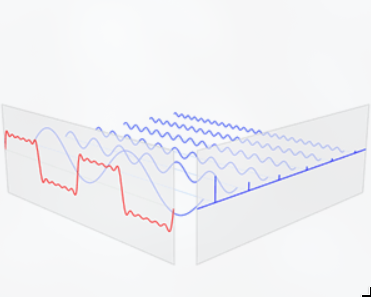
\includegraphics{images/04_01_IllustrazioneTrasformataFourier.png}
    \caption{Interpretazione della trasformata di Fourier}
    \label{fig:04_01_InterpretazioneTrasformataFourier}
\end{figure}

La figura~\ref{fig:04_01_InterpretazioneTrasformataFourier} fornisce una visualizzazione semplificata
di questa interpretazione: il risultato della trasformata è una funzione che \textbf{misura la similarità}
del segnale di ingresso con \textbf{segnali di riferimento a frequenze diverse}.
In particolare:
\begin{itemize}
    \item Se il segnale e l'esponenziale di prova sono \textbf{"simili"}, il prodotto scalare 
        restituisce un \textbf{valore elevato}.
    \item Al contrario, se \textbf{non condividono quella frequenza}, il loro prodotto tende 
        ad \textbf{annullarsi nel calcolo dell'area}.
\end{itemize}

Infine, siccome in generale $X(f) \in \mathbb{C}$, la \textbf{trasformata di un segnale}
presenta un \textbf{modulo} ed una \textbf{fase}. Vale la pena dare
un'interpretazione ad entrambe le componenti:
\begin{itemize}
    \item Il \textbf{modulo} indica \textit{"quanto" contributo} è dato 
        dalla \textit{specifica frequenza}.
    \item La \textbf{fase} indica \textit{"quando"} la specifica frequenza 
        \textit{si presenta nel segnale} (i.e. di \textit{quanto è sfasata rispetto a $t=0$}).
\end{itemize}

\section{Proprietà della trasformata}

Vediamo alcune proprietà della trasformata di Fourier:

\begin{prop}[PROPRIETA' DELLA TRASFORMATA]
    Le proprietà di nostro interesse sono:
    \begin{enumerate}
        \item \textbf{LINEARITA'} 
            \[
                \mathcal{F}[\alpha x_{1}(t) + \beta x_{2}(t)]=
                \alpha \mathcal{F}[x_{1}(t)] + \beta \mathcal{F}[x_{2}(t)]
            \]
        \item \textbf{CAMBIO DI SCALA}
            \[
                \begin{aligned}
                    x(t) &\overset{\mathcal{F}}{ \longrightarrow } X(f) \\ 
                    x(\alpha t) &\overset{\mathcal{F}}{ \longrightarrow } 
                    \frac{1}{|\alpha |}X \left( \frac{f}{|\alpha |} \right)
                \end{aligned}
            \]
        \item \textbf{TRASLAZIONE NEL TEMPO}
            \[
                \begin{aligned}
                    x(t) &\overset{\mathcal{F}}{ \longrightarrow } X(f) \\ 
                    x(t-t_{0}) &\overset{\mathcal{F}}{ \longrightarrow } X(f)e^{-j 2\pi ft_{0}}
                \end{aligned}
            \]
        \item \textbf{TRASLAZIONE IN FREQUENZA}
            \[
                \begin{aligned}
                    x(t) &\overset{\mathcal{F}}{ \longrightarrow } X(f) \\ 
                    x(t)e^{j 2\pi f_{0}t} &\overset{\mathcal{F}}{ \longrightarrow } X(f-f_{0})
                \end{aligned}
            \] 
        \item \textbf{MODULAZIONE} (derivabile dalla traslazione in frequenza) \\
            Con coseno:
            \[
                \begin{aligned}
                    x(t) &\overset{\mathcal{F}}{ \longrightarrow } X(f) \\ 
                    x(t)\cos (2\pi f_{0}t) &\overset{\mathcal{F}}{ \longrightarrow }
                    \frac{1}{2} [ X(f-f_{0}) + X(f+f_{0}) ]
                \end{aligned}
            \]
            Con seno:
            \[
                \begin{aligned}
                    x(t) &\overset{\mathcal{F}}{ \longrightarrow } X(f) \\ 
                    x(t)\sin (2\pi f_{0}t) &\overset{\mathcal{F}}{ \longrightarrow }
                    \frac{1}{2j} [ X(f-f_{0}) - X(f+f_{0}) ]
                \end{aligned}
            \]
        \item \textbf{CONVOLUZIONE}
            \[
                \begin{aligned}
                    x(t) \overset{\mathcal{F}}{ \longrightarrow } X(f) &\text{ , }
                    y(t) \overset{\mathcal{F}}{ \longrightarrow } Y(f) \\ 
                    x(t) \ast y(t) &\overset{\mathcal{F}}{ \longrightarrow } X(f)Y(f)
                \end{aligned}
            \]
        \item \textbf{SIMMETRIA HERMITIANA} Se $x(t)\in \mathbb{R}$, allora 
            $X(-f)=\overline{X(f)}$ (Per cui $\text{Re}[X(f)]$ è \textit{pari}, mentre
            $\text{Im}[X(f)]$ è \textit{dispari}). 
        \item \textbf{AREA DEL SEGNALE}
            \[
                \text{Area}[x(t)] = \int_{-\infty}^{+\infty} x(t) dt = 
                \int_{-\infty}^{+\infty} x(t) e^{-j 2\pi\cdot 0t}dt = X(0) 
            \]
            E, per simmetria, anche:
            \[
                \int_{-\infty}^{+\infty} X(f) df = \int_{-\infty}^{+\infty} X(f) e^{j 2\pi f\cdot 0} dt 
                = x(0)
            \] 
    \end{enumerate}
\end{prop}

\subsection{Esempi di calcolo}

Vediamo ora alcuni esempi di calcolo della trasformata per segnali notevoli.

Per cominciare, vediamo la \textbf{trasformata dell'impulso di Dirac}:

\begin{prop}[TRASFORMATA DELL'IMPULSO]
    Abbiamo:
    \[
        \mathcal{F}[\delta(t)] = 1
    \] 
\end{prop}

Infatti, per la \textit{proprietà rivelatrice dell'impulso}, abbiamo:
\[
    \int_{-\infty}^{+\infty} x(t)\delta(t-t_{0})dt = x(t_{0}) \\ \\
\] 
Per cui segue che:
\[
    \mathcal{F}[\delta(t)] = \int_{-\infty}^{+\infty} \delta(t-0) e^{-j 2\pi ft} dt
    = e^{-j 2 \pi ft}\bigg|_{t=0} = \cos(0) +j \sin(0) = 1
\]

Vediamo ora la trasformata dell'\textbf{esponenziale}:

\begin{prop}[TRASFORMATA DELL'ESPONENZIALE]
    Dato $x(t) = e^{j 2\pi f_{0}t}$, la sua trasformata è:
    \[
        \mathcal{F}\left[ e^{j 2\pi f_{0}t} \right] = \delta(f-f_{0})
    \]
\end{prop}

Questo risultato non deve stupirci: infatti, facendo appello all'interpretazione
che abbiamo dato alla trasformata come \textit{proiezione continua nel dominio della frequenza},
notiamo che un \textbf{segnale esponenziale} è \textbf{caratterizzato da una sola frequenza}, cioè
proprio $f_{0}$.

Inoltre, questo risultato implica anche:

\begin{prop}
    Di conseguenza, se $x(t)= 1 = e^{j 2\pi\cdot 0t}$, allora:
    \[
        \mathcal{F}[1] = \delta(f-0) = \delta(f)
    \] 
\end{prop}

Proseguiamo con la \textbf{trasformata del rettangolo}:

\begin{prop}[TRASFORMATA DEL RETTANGOLO]
    La trasformata di $x(t)=\text{rect}(t)$ è:
    \[
        X(f) = \frac{\sin \pi f}{\pi f} = \text{sinc}(f)
    \] 
\end{prop}

Infatti:
\[   
    \begin{aligned}
        X(f) &= \int_{-\infty}^{+\infty} \overbrace{\text{rect}(t)}^{=1} 
        e^{-j 2\pi ft}dt \\ 
             &= \int_{-\frac{1}{2}}^{\frac{1}{2}} e^{-j 2\pi ft}dt \\
             &= \frac{1}{-j 2\pi f} e^{-j 2\pi ft}\bigg|_{-\frac{1}{2}}^{\frac{1}{2}}
             = \frac{e^{j\pi f} - e^{-j\pi f}}{2j \pi f} \\
             &= \frac{\sin \pi f}{\pi f} = \text{sinc}(f)
    \end{aligned}
\]

\begin{remark}
    E' inoltre utile tenere a mente il fatto che vale anche:
    \[
        \mathcal{F}[\text{sinc}(t)] = \text{rect}(f)
    \] 
    Cioè $\text{sinc}$ e $\text{rect}$ sono \textbf{ciasuno la trasformata dell'altro}.
\end{remark}

Infine, per completezza, vediamo anche la seguente trasformata:

\begin{prop}[ESPONENZIALE NEGATIVO]
    Dato $x(t) = e^{-\alpha t}\mathbf{1}(t)$ (dove $\mathbf{1}(t)$ è il \textit{gradino unitario}
    e $\alpha\in \mathbb{R}^+$), la sua trasformata è:
    \[
        \mathcal{F}[x(t)] = \frac{1}{\alpha + j2\pi f}
    \] 
\end{prop}

Infatti:
\[
    \begin{aligned}
        X(f) &= \int_0^{+\infty} e^{-\alpha t} e^{-j 2\pi ft}dt \\ 
             &= \int_{0}^{+\infty} e^{-(\alpha + j2\pi f)t}dt \\ 
             &= \frac{-1}{\alpha + j 2\pi f} e^{-(\alpha + j 2\pi f)t}\bigg|_{0}^{+\infty} \\ 
             &= \frac{1}{\alpha + j 2\pi f}
    \end{aligned}
\]
Vediamo ora un esempio in cui sfruttiamo il cambio di scala:

\begin{exa}[CAMBIO DI SCALA]
    Consideriamo $x(t) = \text{rect}\left( \frac{t}{10} \right)$.
    Abbiamo semplicemente:
    \[
        X(f) = 10 \text{sinc}(10f)
    \] 
\end{exa}

Abbiamo ottenuto il risultato \textit{semplicemente applicando la proprietà}, senza
dover effettuare \textit{nessun calcolo}.

Vediamo anche degli esempi in cui possiamo sfruttare la traslazione in frequenza:

\begin{exa}[MODULAZIONE]
    Consideriamo un segnale del tipo $x(t)=\cos (2\pi f_{0}t)$. 
    Notiamo che possiamo scriverlo nella forma $x(t) = 1\cdot \cos (2\pi f_{0}t)$.
    Sfruttando la proprietà di \textbf{modulazione} abbiamo quindi:
    \[
        X(f) =\frac{1}{2}\delta(f-f_{0}) + \frac{1}{2}\delta(f+f_{0})
    \]
    Se consideriamo invece $x(t)=\sin (2\pi f_{0}t)$ abbiamo:
    \[
        X(f) = \frac{1}{2j}\delta(f-f_{0}) - \frac{1}{2j}\delta(f+f_{0})
    \] 
\end{exa}

Vediamo anche un esempio in cui \textit{applichiamo diverse proprietà insieme}:

\begin{exa}[ESEMPIO COMPOSTO]
    Consideriamo il segnale seguente:
    \[
        x(t) = \text{sinc}(10t) \cos(6\pi t)
    \] 
    Cominciamo col calcolare la trasformata di $x_{1}(t)=\text{sinc}(10t)$:
    \[
        \mathcal{F}[x_{1}(t)] = \frac{1}{10} \text{rect} \left( \frac{f}{10} \right)
    \] 
    Infine, applicando la proprietà di modulazione a $x_{1}$ con 
    $\cos (6\pi t)=\cos (2\pi\cdot 3t)$ troviamo:
    \[
        \begin{aligned}
            \mathcal{F}[x(t)] &= \frac{1}{2} \left[ 
                \frac{1}{10}\text{rect} \left( \frac{f-3}{10} \right) +
                \frac{1}{10}\text{rect} \left( \frac{f+3}{10} \right)
            \right] \\ 
            &= \frac{1}{20}\text{rect} \left( \frac{f-3}{10} \right) +
            \frac{1}{20}\text{rect} \left( \frac{f+3}{10} \right)
        \end{aligned}
    \] 
\end{exa}

\section{Trasformata e sistemi LTI}

Una proprietà particolarmente utile è quella che riguarda la convoluzione: infatti, se
abbiamo un \textbf{LTI} con un \textbf{segnale di ingresso} $x(t)$, possiamo \textbf{calcolare
la sua uscita} nel \textbf{dominio della frequenza} con \textbf{facilità}, come mostrato nella
figura~\ref{fig:04_02_ConvoluzioneDomTrasformata}.

\begin{figure}[!ht]
    \centering
    \begin{tikzpicture}[
        >=Stealth, 
        thick, 
        font=\sffamily,
        block/.style={
            draw=nord10, 
            rectangle, 
            minimum width=2.5cm, 
            minimum height=1cm, 
            align=center,
            text=nord0
        },
        arrow/.style={->, nord0},
        label/.style={text=nord0, font=\small}
        ]

        % ==========================================
        % PARTE SUPERIORE: DOMINIO DEL TEMPO
        % ==========================================

        % Nodi principali
        \node (xt) at (-4, 2) {\(x(t)\)};
        \node[block] (h) at (0, 2) {\(h(t)\)};
        \node (yt) at (2.65, 2) {\(y(t)\)};
        \node (eq_t) at (4.2, 2) {\(= x(t) * h(t)\)};

        % Frecce
        \draw[arrow] (xt) -- (h);
        \draw[arrow] (h) -- (yt);

        % Annotazioni
        \node[label, above] at (-2.5, 2) {LTI};

        % ==========================================
        % TRASFORMAZIONE DI FOURIER
        % ==========================================

        % Freccia verso il basso
        \draw[arrow, nord11] (0, 1.5) -- (0, -1.5);
        \node[nord11, font=\large\bfseries] at (-0.3, 0) {\(\mathcal{F}\)};

        % ==========================================
        % PARTE INFERIORE: DOMINIO DELLA FREQUENZA
        % ==========================================

        % Nodi principali
        \node (Xf) at (-4, -2) {\(X(f)\)};
        \node[block] (H) at (0, -2) {\(H(f)\)};
        \node (Yf) at (2.65, -2) {\(Y(f)\)};
        \node (eq_f) at (4.5, -2) {\(= H(f) \cdot X(f)\)};

        % Frecce
        \draw[arrow] (Xf) -- (H);
        \draw[arrow] (H) -- (Yf);

    \end{tikzpicture}
    \caption{Sistemi LTI nel dominio della trasformata}
    \label{fig:04_02_ConvoluzioneDomTrasformata}
\end{figure}

Vediamo anche un esempio in cui l'applicazione della proprietà sulla convoluzione
semplifica di molto i calcoli: immaginiamo di voler calcolare la 
\textbf{trasformata del triangolo}. Sappiamo che il triangolo è il risultato della 
\textbf{convoluzione tra due rect}, per cui:
\[
    \text{triang}(t) = \text{rect}(t) \ast \text{rect}(t)
\]

Possiamo allora calcolarne la trasformata come segue:

\begin{exa}[TRASFORMATA DEL TRIANGOLO]
    \[
        \mathcal{F}[\text{triang}(t)] = \mathcal{F}[\text{rect}(t) \ast \text{rect}(t)]
        = \text{sinc}^2(f)
    \] 
\end{exa}

Inoltre, ricordando la relazione tra l'\textbf{area del segnale} e la \textbf{sua trasformata}, 
abbiamo anche:
\[
    \begin{aligned}
        z(t) &= x(t) \ast y(t) \\ 
        \text{Area}[z(t)] &= Z(0) \\ 
                      &= X(f) Y(f) \bigg|_{f=0} \\ 
                      &= X(0) Y(0)
    \end{aligned}
\]

\subsection{Risposta in frequenza}

Possiamo sfruttare la trasformata di Fourier per studiare i sistemi nel 
\textbf{dominio della frequenza invece che nel dominio del tempo}.

\begin{remark}[RISPOSTA IN FREQUENZA]
    Quando l'analisi viene fatta nel \textit{dominio della trasformata di Fourier}
    si parla di \textbf{analisi in frequenza} e \textbf{risposta in frequenza}
    del sistema (cioè la \textit{trasformata} di $h(t)$, ovvero $H(f)$).
\end{remark}

Vediamo alcuni esempi per capire di cosa si tratta.

Consideriamo un generico sistema \textbf{LTI} caratterizzato da una 
\textbf{risposta impulsiva} $h(t)$, come mostrato in figura~\ref{fig:04_03_EsSistemaLTI}.

\begin{figure}[!ht]
    \centering
    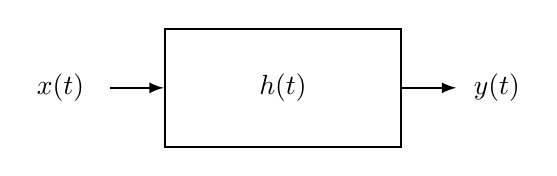
\begin{tikzpicture}[>=latex]
        \node[draw, thick, minimum width=3cm, minimum height=1.5cm] (lti) at (0,0) {$h(t)$};
        \draw[->, thick] (-2.2, 0) -- (lti.west);
        \node[anchor=east] at (-2.4, 0) {$x(t)$};
        \draw[->, thick] (lti.east) -- (2.2, 0);
        \node[anchor=west] at (2.3, 0) {$y(t)$};
    \end{tikzpicture}
    \caption{Esempio di sistema LTI}
    \label{fig:04_03_EsSistemaLTI}
\end{figure}

Per cominciare, consideriamo un ingresso dato da un \textbf{segnale esponenziale}:
\[
    x(t) = e^{j 2\pi f_{0}t}
\]
Calcoliamo l'\textbf{uscita del sistema} nel \textbf{dominio della frequenza}:
\[
    \begin{aligned}
        Y(f) &= H(f) X(f) \\ 
             &= H(f) \delta(f-f_{0})
    \end{aligned}
\]

Ora, per la \textit{proprietà rivelatrice} dell'impulso, abbiamo:
\[
    Y(f) = H(f_{0})\delta(f-f_{0})
\]
Dove $H(f_{0})$ è un \textit{numero (complesso)}. Per cui, applicando l'\textbf{antitrasformata} per 
\textbf{tornare al dominio del tempo}, concludiamo che:
\[
    y(t) = H(f_{0}) e^{j 2\pi f_{0}t}
\]
Notiamo che l'\textbf{uscita del sistema} è semplicemente l'\textbf{ingresso riscalato}
di un fattore $H(f_{0})$.

\begin{remark}[AUTOFUNZIONE PER SISTEMI LTI]
    "Applicare" un \textbf{sistema LTI} $T_h$ ad un \textbf{segnale esponenziale} $x(t)$ è 
    \textbf{equivalente} a \textbf{riscalare il segnale}:
    \[
        T_h \{x(t)\} = \lambda x(t) \text{ , } \lambda = H(f_{0})
    \] 
    Possiamo quindi concludere che tali segnali sono le \textbf{autofunzioni dei sistemi LTI}
    (analoghi agli \textit{autovettori} per le matrici) associati all'
    \textbf{autovalore complesso} $H(f_{0})$.
\end{remark}

Vediamo ora cosa succede se consideriamo lo \textit{stesso sistema LTI}, ma con un
\textbf{ingresso} $x(t)$ \textbf{sinusoidale}:
\[
    x(t) = A \cos(2\pi f_{0}t + \varphi )
\] 

Per cominciare, riscriviamo il segnale di ingresso come segue:
\[
    \begin{aligned}
        x(t) &=\frac{A}{2} e^{j(2\pi f_{0}t + \varphi )} + \frac{A}{2} e^{-j(2\pi f_{0}t + \varphi )} \\ 
             &=\frac{A}{2} e^{j \varphi } e^{j 2\pi f_{0}t} + \frac{A}{2} e^{-j \varphi } e^{-j 2\pi f_{0}t}
    \end{aligned}
\]
Così facendo abbiamo messo in evidenza il fatto che possiamo vederli come \textbf{segnali costanti} 
$\frac{A}{2} e^{j \varphi}$ e $\frac{A}{2} e^{-j \varphi}$ \textbf{traslati} di 
$e^{j 2\pi f_{0} t}$ e $e^{-j 2\pi f_{0} t}$. La trasformata risulta quindi essere:
\[
    X(f) = \frac{A}{2} e^{j \varphi } \delta(f-f_{0}) + \frac{A}{2} e^{-j \varphi } \delta(f+f_{0})
\]

Allora la risposta del sistema è:
\[
    \begin{aligned}
        Y(f) = H(f)X(f) &= \frac{A}{2} H(f) e^{j \varphi } \delta(f-f_{0}) + 
                \frac{A}{2} H(f) e^{-j \varphi } \delta(f+f_{0}) \\ 
             &= \frac{Ae^{j \varphi }}{2} H(f_{0})\delta(f-f_{0}) +
                \frac{Ae^{-j \varphi }}{2} H(-f_{0})\delta(f+f_{0})
    \end{aligned}
\]

Essendo il \textit{segnale reale}, è utile ricordare che la sua trasformata gode di
\textit{simmetria Hermitiana}, per cui $H(-f_{0})=\overline{H(f)}$ e la risposta risulta:
\[
   Y(f) = \frac{Ae^{j \varphi }}{2} H(f_{0})\delta(f-f_{0}) +
          \frac{Ae^{-j \varphi }}{2} \overline{H(f_{0})}\delta(f+f_{0}) 
\]
Ricordando che $H(f_{0})$ è un \textbf{numero complesso}, scriviamo:
\[
    Y(f) = \frac{Ae^{j \varphi }}{2} |H(f_{0})|e^{j\angle H(f_{0})} \delta(f-f_{0}) +
          \frac{Ae^{-j \varphi }}{2} |H(f_{0})|e^{-j\angle H(f_{0})} \delta(f+f_{0}) 
\]
Raccogliendo troviamo:
\[
    Y(f) = \frac{A|H(f_{0})|}{2} \left[ e^{j(\varphi + \angle H(f_0)) } \delta(f-f_{0}) +  
           e^{-j (\varphi + \angle H(f_0)) } \delta(f+f_{0}) \right]
\]

Ora, antitrasformando per \textit{tornare nel dominio del tempo}, troviamo:
\[
    \begin{aligned}
        y(t) &= \frac{A|H(f_{0})|}{2} \left[ e^{j(\varphi + \angle H(f_0))} e^{j 2\pi f_{0}t} +
                e^{-j(\varphi + \angle H(f_0))} e^{-j 2\pi f_{0}t} \right] \\ \\
             &= \frac{A|H(f_{0})|}{2} \underbrace{ \left[ e^{j(2\pi f_{0}t + \varphi + \angle H(f_0))} +
             e^{-j(2\pi f_{0}t + \varphi + \angle H(f_0))} \right] }_{=2\cos 
                (2\pi f_{0}t + \varphi + \angle H(f_0) )} \\ \\
             &= A|H(f_{0})| \cos (2\pi f_{0}t + \varphi + \angle H(f_0) )
    \end{aligned}
\]

\begin{remark}[RISPOSTA SISTEMI LTI A INGRESSI SINUSOIDALI]
    La \textbf{risposta} di un \textbf{sistema LTI} ad un \textbf{ingresso sinusoidale}
    di \textbf{frequenza} $f_{0}$ è un altro \textbf{segnale sinusoidale}, con 
    la \textbf{stessa frequenza}, ma \textbf{modulo} e \textbf{fase modificati}:
    \begin{itemize}
        \item Il \textbf{modulo} è \textbf{scalato} di un fattore $|H(f_{0})|$.
        \item Alla \textbf{fase} è  sommato un contributo dato da $\angle H(f_{0})$.
    \end{itemize}
\end{remark}

Infine, dato che in generale $Y(f)\in \mathbb{C}$, essa può presentare una 
\textbf{fase}, che merita di essere discussa.
In particolare, è utile definire la seguente quantità:

\begin{definition}[RITARDO DI GRUPPO]
    Il \textbf{ritardo di gruppo} è il \textbf{ritardo subito} dal 
    \textbf{segnale} al \textbf{variare delle frequenze che lo compongono}:
    \[
        \tau_g(f) \coloneqq -\frac{1}{2\pi} \frac{d}{df} \angle Y(f)
    \] 
\end{definition}

Questa quantità è importante perchè:

\begin{remark}[RITARDO DI GRUPPO E DISTORSIONE]
    Se il ritardo di gruppo è \textbf{costante} su 
    \textbf{al variare della frequenza del segnale}, possiamo concludere
    che \textbf{il sistema non ha introdotto una distorsione}, cioè ha 
    \textbf{preservato la forma} del segnale.

    Al contrario, se \textbf{varia con la frequenza}, si verifica una 
    \textbf{distorsione della forma d'onda} a causa della 
    \textbf{diversa velocità di propagazione} 
    delle \textbf{diverse componenti frequenziali}.
\end{remark}

\subsection{Banda e larghezza di banda}

Dato un segnale, possiamo definire la sua \textbf{banda}:

\begin{definition}[BANDA DI UN SEGNALE]
    La banda di un segnale $x(t)$ è l'
    \textbf{intervallo di frequenze non negative} 
    per cui la sua \textbf{trasformata} risulta \textbf{non nulla}:
    \[
        \mathcal{B}_x \coloneqq \{f\in \mathbb{R}^+\}   : X(f) \ne 0 
    \] 
\end{definition}

E' da notare che consideriamo \textbf{solo le frequenze positive}. Questo perchè,
come abbiamo visto, se il segnale è reale sappiamo che $X(-f) = \overline{X(f)}$,
quindi la \textbf{parte reale della trasformata è pari} e ci \textit{basta considerare
le frequenze positive} (lo \textit{spettro negativo sarà uguale}).

Inoltre, possiamo anche \textit{estendere questo concetto ai sistemi}:

\begin{definition}[BANDA DI UN SISTEMA]
    Dato un \textbf{sistema} $h$, ne definiamo la \textbf{banda passante} $B_h$
    a partire dalla \textbf{risposta in frequenza}:
    \[
        \mathcal{B}_h = \{f\in \mathbb{R}^+ : H(f) \ne 0 \}
    \] 
\end{definition}

Si definisce inoltre la \textbf{larghezza di banda}:

\begin{definition}[LARGHEZZA DI BANDA]
    Data la \textbf{banda} di un segnale (o la \textit{banda passante di un sistema})
    $\mathcal{B}= [f_{1},f_{2}]  $, la \textbf{larghezza di banda} $B$ 
    (o \textit{bandwidth}) è:
    \[
        B = f_{2} - f_{1}
    \] 
\end{definition}

La figura~\ref{fig:04_04_EsempioBandaLarghezza} mostra la \textbf{banda} e la 
\textbf{larghezza di banda} per un segnale di esempio.

\begin{figure}[!ht]
    \centering
    \begin{tikzpicture}[xscale=1.5, yscale=2, >=stealth, font=\small]
        % Assi
        \draw[->, thick, nord0] (-4, 0) -- (4.5, 0) node[right, font=\bfseries] {\(f\)};
        \draw[->, thick, nord0] (0, -0.2) -- (0, 1.5) node[above, font=\bfseries] {\(X(f)\)};

        % Spettro del segnale (esempio di un passa-banda)
        % Parte positiva (quella che definisce la banda)
        \draw[very thick, nord10] (1, 0) -- (1, 1) -- (3, 1) -- (3, 0);
        % Parte negativa (simmetrica, tratteggiata per far capire che non la contiamo)
        \draw[very thick, nord10, dashed] (-3, 0) -- (-3, 1) -- (-1, 1) -- (-1, 0);

        % Evidenziazione della Banda (Area sotto la parte positiva)
        \fill[nord14, opacity=0.3] (1, 0) rectangle (3, 1);

        % Etichette sugli assi
        \draw[nord0, thick] (0.95, 0) -- (1.05, 0) node[below=2pt, nord0] {\(f_1\)};
        \draw[nord0, thick] (2.95, 0) -- (3.05, 0) node[below=2pt, nord0] {\(f_2\)};
        \draw[nord0, thick] (0, 1) -- (-0.05, 1) node[left, nord0] {\(\max\)};

        % Parentesi graffa per la Banda B_x
        \draw[decorate, decoration={brace, amplitude=5pt, mirror}, nord11, thick] 
            (1, -0.4) -- (3, -0.4) node[midway, below=6pt, nord11] 
            {Banda \(B_x = \{f \in \mathbb{R}^+ : X(f) \neq 0\}\)};

        % Frecce per la Larghezza di Banda
        \draw[<->, thick, nord12] (1, 1.2) -- (3, 1.2) 
            node[midway, above, nord12] {Larghezza di banda \(B = f_2 - f_1\)};

        % Nota sulla parte negativa
        \node[align=center, font=\footnotesize, nord3] at (-2, 0.5) 
            {Spettro negativo \\ simmetrico};
    \end{tikzpicture}
    \caption{Esempio: banda e larghezza di banda di $x(t) = \text{sinc}(t) e^{j 2\pi f_{0}t}$}
    \label{fig:04_04_EsempioBandaLarghezza}
\end{figure}

A questo punto, è importante notare che in moltissimi casi la definizione di banda 
come \textit{intervallo in cui la trasformata è diversa da zero} 
porterebbe ad avere una \textbf{banda infinita}, mentre dal \textit{punto di vista pratico} 
quello che interessa è l’\textbf{intervallo in cui la trasformata è \textit{significativamente}
diversa da zero}.

Con questo in mente, consideriamo due \textbf{definizioni alternative}
di \textbf{larghezza di banda}:

\begin{definition}[LARGHEZZA DI BANDA - DEF. ALTERNATIVE]
    Consideriamo le seguenti due definizioni:
    \begin{enumerate}
        \item \textbf{Primo zero}: ci limitiamo al \textit{primo zero della trasformata}.
            \[
                B = \text{min } \{ f > 0 \text{ t.c } H(f) = 0 \}  
            \] 
        \item Basata sull'\textbf{ampiezza} (in \textit{decibel}):
            \[
                B = \text{min } \left\{ f > 0 \text{ t.c. } \left| \frac{H(f)}{H(0)} \right| 
                = 10^{- \frac{A}{20}} \right\}
            \] 
    \end{enumerate}
\end{definition}

Per quanto riguarda la seconda definizione, ricordiamo la \textit{definizione di decibel}
e consideriamo la figura~\ref{fig:04_05_EsempioDefPraticaBanda} per un esempio visivo.

\begin{figure}[!ht]
    \centering
    \begin{tikzpicture}
        \begin{axis}[
            width=12cm, height=7.5cm,
            xmin=0, xmax=2,
            ymin=-100, ymax=5,
            xtick={0, 0.2, 0.4, 0.6, 0.8, 1, 1.2, 1.4, 1.6, 1.8, 2},
            ytick={0, -10, -20, -30, -40, -50, -60, -70, -80, -90, -100},
            xlabel={\(f\) (Hz)},
            ylabel={\(|H(f)|\) (dB)},
            axis line style={nord0, thick},
            tick style={nord0, thick},
            tick label style={nord0},
            label style={nord0, font=\bfseries},
            grid=major,
            grid style={nord4, dashed},
            clip=false
            ]

            % --- 1. Curva della risposta in frequenza (approssimata per riprodurre la forma) ---
            \addplot [
                nord10, very thick, smooth
                ] coordinates {
                    (0, 0) (0.1, 0) (0.2, 0) (0.3, 0) (0.35, -0.1)
                    (0.4, -0.5) (0.45, -1.2) (0.5, -3) 
                    (0.55, -8) (0.6, -25) (0.652, -30) 
                    (0.68, -35) (0.75, -38) (0.82, -45) (0.85, -40) 
                    (0.87, -40) (0.9, -45) (1.0, -55) (1.05, -60) 
                    (1.1, -55) (1.2, -60) (1.25, -70) 
                    (1.3, -60) (1.4, -65) (1.45, -90) 
                    (1.5, -65) (1.62, -50) (1.7, -100)
                };

            % --- 2. Linee orizzontali e verticali per le larghezze di banda ---

            % Banda a 3 dB (B_3dB)
            \draw[dashed, nord3, thick] (axis cs:0, -3) -- (axis cs:0.5, -3);
            \draw[dashed, nord3, thick] (axis cs:0.5, -3) -- (axis cs:0.5, -101);

            % Banda a 40 dB (B_40dB)
            \draw[dashed, nord3, thick] (axis cs:0, -40) -- (axis cs:0.77, -40);
            \draw[dashed, nord3, thick] (axis cs:0.77, -40) -- (axis cs:0.77, -101);

            % Banda a 60 dB (B_60dB)
            \draw[dashed, nord3, thick] (axis cs:0, -60) -- (axis cs:1.05, -60);
            \draw[dashed, nord3, thick] (axis cs:1.05, -60) -- (axis cs:1.05, -101);

            % --- 3. Etichette testuali ---

            % Etichette in alto a sinistra
            \node[anchor=north, nord0, font=\footnotesize] at (axis cs:0.2, -3) {\(B_{3dB}\)};
            \node[anchor=north, nord0, font=\footnotesize] at (axis cs:0.2, -40) {\(B_{40dB}\)};
            \node[anchor=north, nord0, font=\footnotesize] at (axis cs:0.2, -60) {\(B_{60dB}\)};

        \end{axis}

    \end{tikzpicture}
    \caption{Larghezza di banda basata sull'attenuazione dell'ampiezza}
    \label{fig:04_05_EsempioDefPraticaBanda}
\end{figure}

\begin{remark}
    Il \textbf{decibel} è utilizzato per quantificare l'\textbf{attenuazione} 
    del segnale ed è definito come:
    \[
        A_{dB} = 20 \log_{10} \left( \frac{|H(f)|}{H(0)} \right)
    \] 
    Spesso si usano come valori di $A$:
    \begin{itemize}
        \item $A=3dB$: valore di \textbf{half-power} (si ha $10^{-3/20} \approx 1/\sqrt{2}$)
        \item $A=40dB$: attenuazione dell'ampiezza di $100$ volte.
        \item $A=60dB$: attenuazione dell'ampiezza di $1000$ volte.
    \end{itemize}
\end{remark}


\section{Teorema di Parseval}

Un teorema particolarmente importante è il seguente:

\begin{theorem}[TEOREMA DI PARSEVAL]
    Dati due \textbf{segnali} $x(t)$ e $y(t)$, vale:
    \[
        \int_{-\infty}^{+\infty} x(t) \overline{y(t)} dt = 
        \int_{-\infty}^{+\infty} X(f) \overline{Y(f)} df  
    \] 
\end{theorem}

Vediamo un esempio in cui questo teorema può risultare utile:

\begin{exa}[APPLICAZIONE TH. PARSEVAL]
    Consideriamo:
    \[
        \begin{aligned}
            x(t) = \text{sinc}(10t) & & y(t) = \text{sinc}(5t)
        \end{aligned}
    \] 
    L'integrale seguente è particolarmente complicato da calcolare:
    \[
        \int_{-\infty}^{+\infty} \frac{\sin 10\pi t}{10\pi t} \frac{\sin 5\pi t}{5\pi t} dt
    \] 
    Possiamo tuttavia sfruttare il teorema di Parseval per calcolare:
    \[
        \begin{aligned}
            \int_{-\infty}^{+\infty} X(f) \overline{Y(f)} df &= 
            \frac{1}{50} \int_{-\infty}^{+\infty} \text{rect} \left( \frac{f}{10} \right)
            \overline{ \text{rect} \left( \frac{f}{5} \right) } df \\ 
            &= \frac{1}{50} \int_{-\infty}^{+\infty} \text{rect} \left( \frac{f}{10} \right)
            \text{rect} \left( \frac{f}{5} \right) df \\ 
            &= \frac{1}{50} \int_{-\infty}^{+\infty} \text{rect} \left( \frac{f}{5} \right) \\ 
            &= \frac{5}{50} = \frac{1}{10}
        \end{aligned}
    \] 
    Dove abbiamo sfruttato il fatto che:
    \begin{itemize}
        \item Il \textbf{congiugato} di un segnale \textbf{reale} 
            rimane il \textbf{segnale stesso}.
        \item La \textbf{moltiplicazione di due rect} risulta in un \textbf{rect}
            nella \textbf{zona di intersezione} fra i due.
    \end{itemize}
\end{exa}

Inoltre osserviamo che, se $y(t) = x(t)$, dal teorema segue che:

\begin{prop}[COROLLARIO TH. PARSEVAL]
    \[
        \int_{-\infty}^{+\infty} x(t) \overline{x(t)} dt = 
        \int_{-\infty}^{+\infty} |x(t)|^2 dt =
        \int_{-\infty}^{+\infty} X(f) \overline{X(f)} df =
        \int_{-\infty}^{+\infty} |X(f)|^2 df
    \] 
\end{prop}

\section{Trasformata di Fourier a tempo discreto}

Vediamo ora come possiamo \textit{generalizzare la trasformata di Fourier} per 
poterla \textbf{applicare} anche a \textbf{segnali a tempo discreto}.

\begin{definition}[TRASFORMATA DI FOURIER A TEMPO DISCRETO]
    Dato un \textbf{segnale} $x(nT)$ ($n\in \mathbb{Z}$) a \textbf{tempo discreto}, la sua
    \textbf{trasformata di Fourier} $\mathcal{F}[x(nT)]$ è definita come segue:
    \[
        \mathcal{F}[x(nT)] = X(f) = \sum_{n=-\infty}^{+\infty} T x(nT) e^{-j 2\pi fnT}
    \] 
\end{definition}

\begin{remark}[CONTINUITA' DELLA FREQUENZA]
    Anche se il segnale originale era in tempo discreto, la sua trasformata
    è \textbf{comunque in frequenze continue} $f\in \mathbb{R}$.
\end{remark}

Ora espandiamo la sommatoria per notare un particolare:
\[
    \begin{aligned}
        X(f) = \ldots +& \underbrace{ Tx(-2T) e^{j 2\pi f\cdot 2T} }_{n=-2} + 
                  \underbrace{ Tx(-T) e^{j 2\pi f\cdot T} }_{n=-1}
                 + Tx(0) \\ 
                 +& \underbrace{ Tx(T) e^{-j 2\pi f\cdot T} }_{n=1} + 
                  \underbrace{ Tx(2T) e^{-j 2\pi f\cdot 2T} }_{n=2} + \ldots 
    \end{aligned}
\]

Notiamo che:
\begin{itemize}
    \item I termini associati ad $n= \pm 1$ sono \textbf{periodici} di periodo $T_{1} = \frac{1}{T}$.
    \item I termini associati ad $n= \pm 2$ sono \textbf{periodici} di periodo $T_{2} = \frac{1}{2T}$.
\end{itemize}

Andando avanti, noteremmo che, in generale, i termini associati ad $n= \pm k$ sono 
\textbf{periodici} di periodo $T_{k} = \frac{1}{kT}$. La cosa importante è che
\textbf{tutti questi termini} si \textbf{ripetono} con \textbf{periodo comune} $\frac{1}{T}$.

Vale quindi il seguente fatto (\textbf{solo per la trasformata a
tempo discreto}, non era vero per quella a tempo continuo):

\begin{remark}[PERIODICITA']
    Per segnali a \textbf{tempo discreto}, la \textbf{trasformata} di Fourier 
    risulta essere \textbf{periodica} di \textit{periodo}:
    \[
        T_f = \frac{1}{T}
    \] 
\end{remark}

Inoltre, anche a tempo discreto possiamo definire la trasformata inversa:

\begin{definition}[TRASFORMATA INVERSA A TEMPO DISCRETO]
    Il segnale \textit{"originale"} può essere ottenuto con la trasformazione inversa:
    \[
        x(nT) = \int_{- \frac{1}{2T}}^{\frac{1}{2T}} X(f) e^{j 2\pi fnT} df
    \] 
\end{definition}

E' da notare che:

\begin{remark}
    Essendo $X(f)$ \textbf{periodica} per un segnale discreto, possiamo \textbf{ricostruire}
    il \textbf{segnale originale} $x(nT)$ \textbf{integrando} su 
    \textbf{un solo periodo} $T_f$.

    In generale, avremmo potuto scegliere \textit{qualsiasi intervallo} di 
    \textit{ampiezza} $T_f$ (e.g. $[0, \frac{1}{T}]$); quello scelto nella 
    defininizione è \textit{più comune} data la sua \textit{simmetria rispetto
    all'origine}.
\end{remark}

\subsection{Esempi di calcolo}

Vediamo ora alcuni esempi:

Per cominciare, consideriamo il segnale:
\[
    x(nT) = \text{rect} \left(\frac{nT}{5T} \right)
\]

Essendo $\text{rect}(t)$ definito se $|t|\le \frac{1}{2}$, abbiamo:
\[
    x(nT) = \begin{cases}
        1 & |n| \le 2 \\ 
        0 & |n| > 2
    \end{cases}
\]

Il segnale è mostrato in figura:

\begin{figure}[!ht]
    \centering
    \begin{tikzpicture}[>=stealth, font=\small]

        % Assi cartesiani
        \draw[->, thick, nord0] (-4.5, 0) -- (4.5, 0) node[right, font=\bfseries] {\(nT\)};
        \draw[->, thick, nord0] (0, -0.2) -- (0, 1.3) node[above, font=\bfseries] {\(x(nT)\)};

        % Linea tratteggiata di guida per y=1
        \draw[dashed, nord3, thick] (-2.5, 1) -- (2.5, 1);

        % Steli e punti per n dove x(nT) = 1 (da -2 a 2)
        \foreach \x in {-2, -1, 0, 1, 2} {
            \draw[nord8, very thick] (\x, 0) -- (\x, 1);
            \fill[nord10] (\x, 1) circle (2.5pt);
        }

        % Punti per n dove x(nT) = 0 (fuori dall'intervallo)
        \foreach \x in {-4, -3, 3, 4} {
            \fill[nord10] (\x, 0) circle (2.5pt);
        }

        % Etichette sull'asse x (nT)
        \foreach \x in {-4, -3, -2, -1, 1, 2, 3, 4} {
            \draw[nord0, thick] (\x, 0) -- (\x, -0.05) node[below, nord0] {\(\frac{\x}{5}\)};
        }
        \draw[nord0, thick] (0, 0) -- (0, -0.05) node[below, nord0] {\(0\)};
        
        % Etichetta sull'asse y
        \draw[nord0, thick] (0, 1) -- (-0.05, 1) node[left, nord0] {\(1\)};

        % Parentesi graffa per evidenziare l'intervallo |n| <= 2
        \draw[decorate, decoration={brace, amplitude=5pt, mirror}, nord11, thick] 
            (-2, -0.75) -- (2, -0.75) node[midway, below=6pt, nord11] {\(|n| \le 2\)};

    \end{tikzpicture}
    \caption{Esempio di segnale rect a tempo discreto}
\end{figure}

Calcoliamone la trasformata:
\[
    \begin{aligned}
        X(f) =& T e^{-j 2\pi f\cdot (-2T)} + 
                T e^{-j 2\pi f\cdot (-T)} + 
                T \\ 
             +& T e^{-j 2\pi f\cdot T} + 
                T e^{-j 2\pi f\cdot 2T)} 
    \end{aligned}
\]

Raccogliendo i termini troviamo:
\[
    \begin{aligned}
        X(f) = T \big[ 1 + &\left( e^{j 2\pi f\cdot 2T} + e^{-j 2\pi f\cdot 2T} \right) \\ 
                        &\left( e^{j 2\pi f\cdot T} + e^{-j 2\pi f\cdot T} \right) \big]
    \end{aligned}
\]

Per cui concludiamo:
\[
    X(f) = T\left[ 1 + 2\cos(2\pi fT) + 2\cos(4\pi fT)  \right]
\]

E' facile intuire che il risultato generale è:

\begin{prop}[TRASFORMATA DEL RECT A T.D.]
    In \textbf{generale}, la trasformata di un segnale rect del tipo
    \[
        x(nT) = \text{rect} \left( \frac{nT}{LT} \right)
    \] 
    Con $L=2M+1$, $M\in \mathbb{N}$, è:
    \[
        X(f) = T \left[ 1 + 2 \sum_{n=1}^M \cos(2\pi fnT) \right]
    \] 
\end{prop}

Consideriamo ora $x(nT) = \left( \frac{1}{3} \right)^{nT} \mathbf{1}(nT)$, mostrato
anche in figura:

\begin{figure}[!ht]
    \centering
    \begin{tikzpicture}[>=stealth, font=\small]

        % Assi cartesiani
        \draw[->, thick, nord0] (-2.5, 0) -- (5.5, 0) node[right, font=\bfseries] {\(nT\)};
        \draw[->, thick, nord0] (0, -0.1) -- (0, 1.4) node[above, font=\bfseries] {\(x(nT)\)};

        % Steli e punti per n >= 0 (valori calcolati: 1, 1/3, 1/9, 1/27, 1/81)
        \foreach \n/\val in {0/1, 1/0.333, 2/0.111, 3/0.037, 4/0.012} {
            \draw[nord8, very thick] (\n, 0) -- (\n, \val);
            \fill[nord10] (\n, \val) circle (2.5pt);
        }

        % Punti per n < 0 (dove 1(nT) = 0)
        \foreach \n in {-1, -2} {
            \fill[nord10] (\n, 0) circle (2.5pt);
        }

        % Etichette sull'asse x (nT)
        \foreach \x/\label in {-2/-2T, -1/-T, 0/0, 1/T, 2/2T, 3/3T, 4/4T} {
            \draw[nord0, thick] (\x, 0) -- (\x, -0.05) node[below, nord0] {\(\label\)};
        }

        % Etichette sull'asse y
        \draw[nord0, thick] (0, 1) -- (-0.05, 1) node[left, nord0] {\(1\)};
    \end{tikzpicture}
    \caption{Esempio di sequenza esponenziale}
\end{figure}

Applicando la trasformata, troviamo $X(f)=0$ per $n<0$, mentre per $n\ge 0$ abbiamo:
\[
    X(f) = \sum_{n=0}^{+\infty} \left( \frac{1}{3} \right)^n e^{-j 2\pi fnT}
\]

Riscriviamolo nella forma:
\[
    X(f) = \sum_{n=0}^{+\infty} \left( \frac{1}{3} e^{-j 2\pi fT} \right)^n
\]

Essendo questa una \textbf{serie geometrica} di ragione $r=\frac{1}{3} e^{-j 2\pi fT}$ 
con $|r|<1$, troviamo che la serie converge a:
\[
    X(f) = \frac{1}{1 - \frac{1}{3}e^{-j 2\pi fT} }
\]

A questo punto è facile intuire il \textbf{risultato generale} per 
una sequenza esponenziale generica:

\begin{prop}[TRASFORMATA DELLA SEQUENZA ESPONENZIALE]
    In generale, la trasformata di $x(nT) = a^{nT} \mathbf{1}(nT)$
    \[
        X(f) = \frac{1}{1 - ae^{-j 2\pi fT} } \text{ , }|a|<1
    \] 
\end{prop}
